\chapter{Weather Simulation at MeteoSwiss}


\section{Introduction}
COSMO, the Consortium for Small-scale Modeling \cite{label47}, is an association seeking to develop, improve and maintain a non-hydrostatic limited-area atmospheric model, the COSMO-model. This is the base for many national weather prediction services in Europe. \\
The consortium was established in 1998 by DWD (Germany) and MeteoSwiss (Switzerland). Over the years, weather services and organizations such as ZGeoBw (Germany), ITAF ReMet/CIRA/ARPAE, ARPA Piemont (Italy), HNMS (Greece), IMGW (Poland), IMS (Israel), NMA (Romania) and RHM (Russia) have joined. In addition to meteorological services, there are also academic communities involved, namely the Climate Limited-Area Modeling (CLM) that extended the model for long-term simulations and Universities maintaining their own extensions. The Karlsruhe Insitute for Technology (KIT) extended the model to account for the interactions of gases and aerosols within the state of the atmosphere. \\
The COSMO-model was initially based on DWDs "Lokal-Modell" (Local Model) and further refined and improved in joint collaboration by the COSMO members.


\paragraph{Structure}
A time integration cycle illustrated in figure \ref{fig:cosmo-the-cosmo-model} can be broken down into different tasks and execution phases \cite{label49}. The first steps prepares the input data for processing. The physics step accounts for the physical processes that are not resolved by the 3-dimensional numerical grid (vertical diffusion (turbulences), cloud and precipitation formation (condensation), convection, radiation and soil processes). \\
The dynamical core, consisting of the dynamics and relaxations phase, is the main computational challenge of the weather model. It is formulated in terms of stencil programs applied on the highly regular, three dimensional data grid. Therefore, we focus on this part of the model. \\
The nudging step takes care of the convergence of the computed model values and the actual observations from the observation stations. Finally there is post-processing going on and a cleanup to be ready for the next iteration step.
\begin{figure}[h]
	\centering
	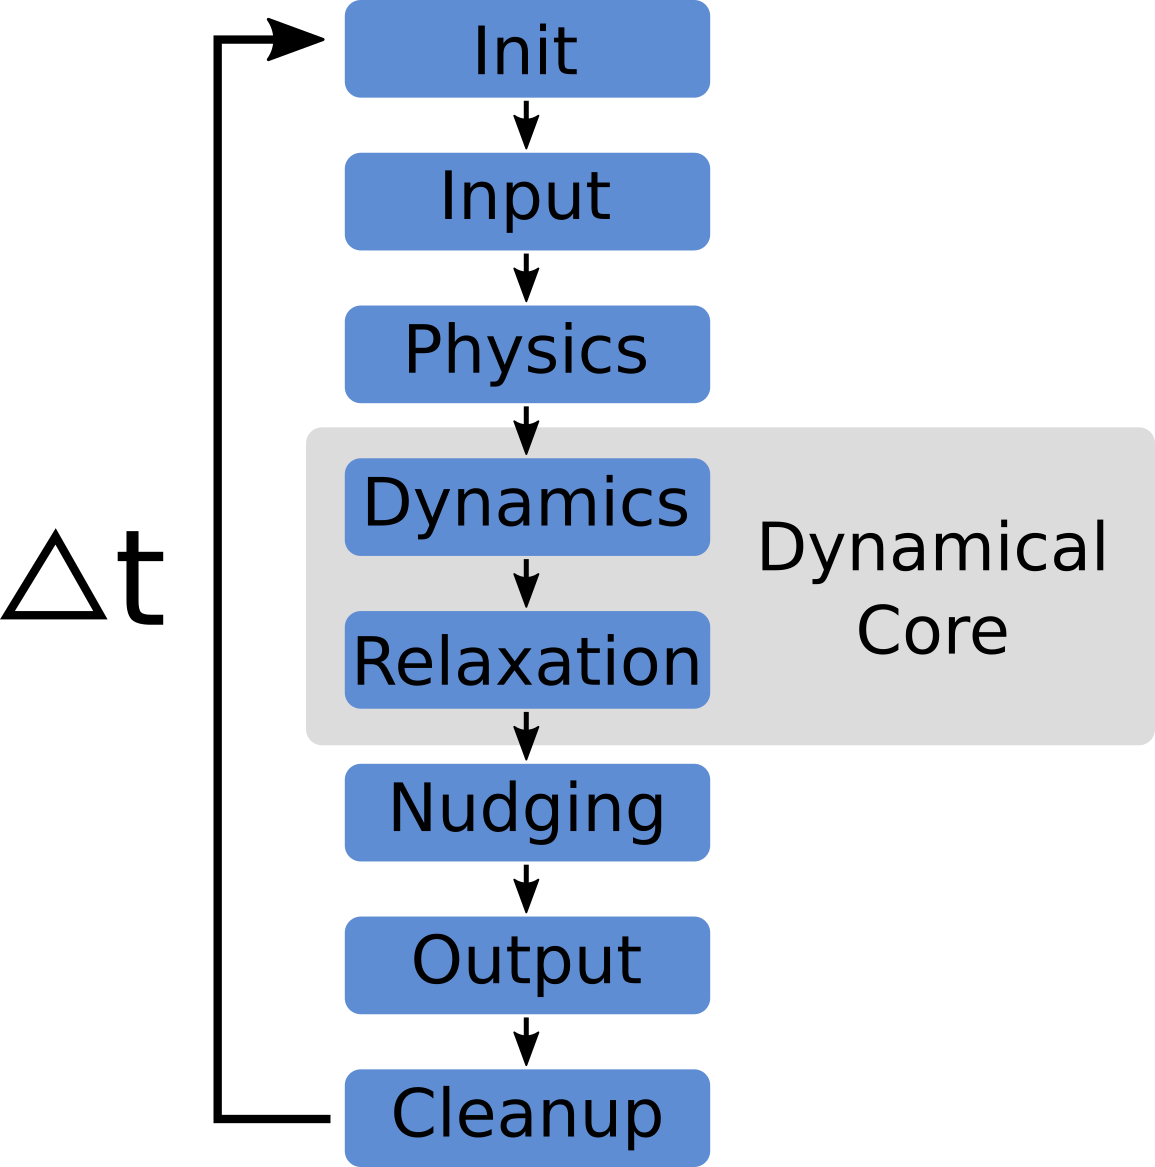
\includegraphics[height=12em]{drawings/cosmo-the-cosmo-model.png}
	\caption{The COSMO Model: Structure of a the time integration interval.}
	\label{fig:cosmo-the-cosmo-model}
\end{figure}


\paragraph{Model Instances (MeteoSwiss Specific)}
MeteoSwiss does not rely on a single instance of the weather model, but rather follows the approach of subdivisions of the forecast into different set of problems \cite{label51}. There are various grid resolution instances and simulation durations shown in figure \ref{fig:cosmo-prediction}, which gives them the ability to better predict longer-term, mid-term and short-term weather constellations in the very challenging topological Alpine region. These grid resolutions define the computational domain of the problem since all stencil operators are applied to each individual grid point.
\begin{figure}[h]
	\centering
	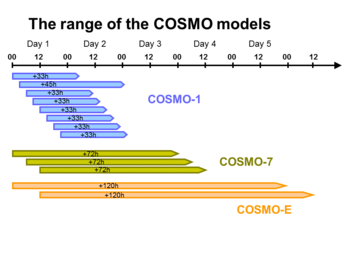
\includegraphics[height=12em]{images/cosmo-prediction.png}
	\caption{Range of COSMO models with their forecast horizon and number of runs per day. \textit{meteoswiss.admin.ch}}
	\label{fig:cosmo-prediction}
\end{figure}


\subparagraph{COSMO-1}
The COSMO-1 instance is a high-resolution version with a grid-box size of 1.1km (0.01\degree) spread over the Alpine region. It is able to predict precipitation, temperature, wind as seen in figure \ref{fig:cosmo-1} and numerous other meteorological parameters. The number of grid points is 1158x774 horizontally and 80 in the vertical dimension. The model topography reaches 4268 meters above sea level. Every grid point is updated in a time integration interval of 10 seconds.
\begin{figure}[h]
	\begin{minipage}{.24\columnwidth}
		\centering
		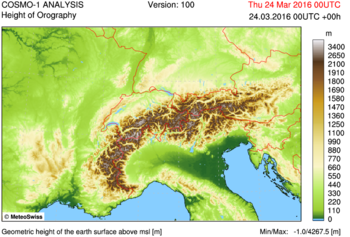
\includegraphics[height=5em]{images/cosmo-1-general.png}
		\label{fig:cosmo-1-general}
	\end{minipage}
	\begin{minipage}{.24\columnwidth}
		\centering
		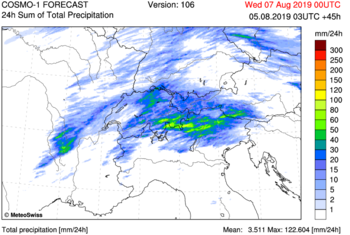
\includegraphics[height=5em]{images/cosmo-1-precipitation.png}
		\label{fig:cosmo-1-precipitation}
	\end{minipage}
	\begin{minipage}{.24\columnwidth}
		\centering
		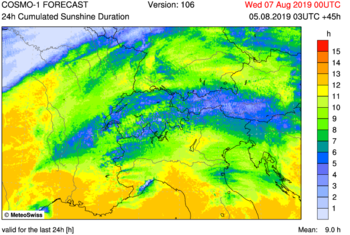
\includegraphics[height=5em]{images/cosmo-1-sunshine-duration.png}
		\label{fig:cosmo-1-sunshine-duration}
	\end{minipage}
	\begin{minipage}{.24\columnwidth}
		\centering
		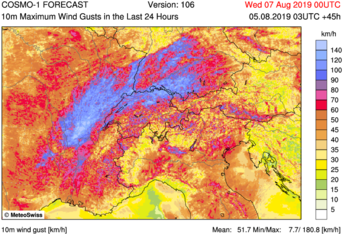
\includegraphics[height=5em]{images/cosmo-1-10m-max-wind-guts.png}
		\label{fig:cosmo-1-10m-max-wind-guts}
	\end{minipage}
	\caption{COSMO-1 example model parameters: Height of Orography, Sum of total Precipitation (Prediction), 24h Sum of Sunshine Hours (Prediction), 10m Above Ground Maximum Wind Guts (Past) (from left to right), \textit{meteoswiss.admin.ch}}
	\label{fig:cosmo-1}
\end{figure}


\subparagraph{COSMO-E}
The COSMO-E models purpose is to improve the reliability of the short to medium range forecast for highly localized weather events. It is a collection of 21 different forecasts that are being executed twice a day. \\
It covers the whole Alpine region, but with a lower resolution in comparison to the COSMO-1 instance. It uses grid box sizes of 2.2km and 582x390 horizontal grid points and 60 vertical layers.
\begin{figure}[h]
	\begin{minipage}{.32\columnwidth}
		\centering
		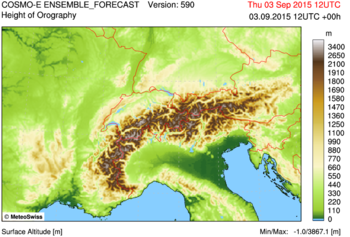
\includegraphics[height=8em]{images/cosmo-m-general.png}
		\label{fig:cosmo-m-general}
		\vspace{-1em}
	\end{minipage}
	\begin{minipage}{.32\columnwidth}
		\centering
		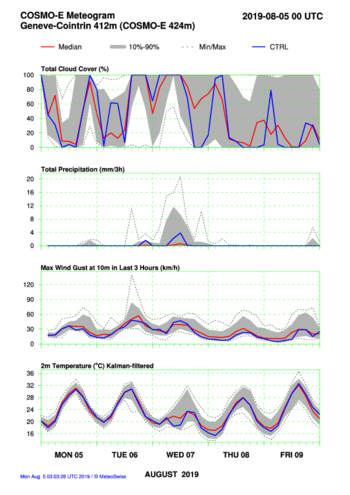
\includegraphics[height=8em]{images/cosmo-m-meteograph-geneve.png}
		\label{fig:cosmo-m-meteograph-geneve}
	\end{minipage}
	\begin{minipage}{.32\columnwidth}
		\centering
		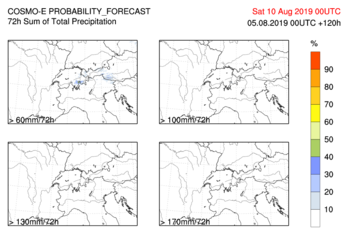
\includegraphics[height=8em]{images/cosmo-m-probability-forecast.png}
		\label{fig:cosmo-m-probability-forecast}
		\vspace{-1em}
	\end{minipage}
	\caption{COSMO-E example model parameters: Height of Orography, Meteogram for Geneva-Cointrin, Probability Forecast (from left to right), \textit{meteoswiss.admin.ch}}
\end{figure}


\subparagraph{COSMO-7}
The COSMO-7 instance with a grid box size of 6.6km (0.06\degree) is a low-resolution version with the aim of covering central and western Europe. The predictions are being run four times a day over a grid of size 393x338 horizontally and 60 vertical units.
\begin{figure}[h]
	\begin{minipage}{.32\columnwidth}
		\centering
		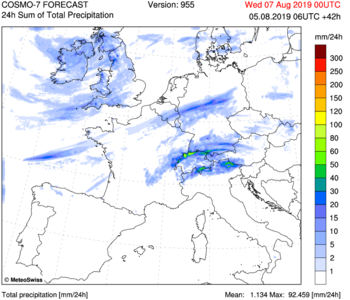
\includegraphics[height=8em]{images/cosmo-7-precipitation.png}
		\label{fig:cosmo-7-precipitation}
	\end{minipage}
	\begin{minipage}{.32\columnwidth}
		\centering
		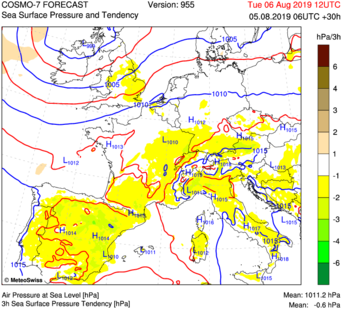
\includegraphics[height=8em]{images/cosmo-7-forecast.png}
		\label{fig:cosmo-7-forecast}
	\end{minipage}
	\begin{minipage}{.32\columnwidth}
		\centering
		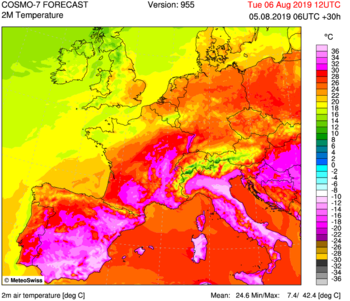
\includegraphics[height=8em]{images/cosmo-7-temperature.png}
		\label{fig:cosmo-7-temperature}
	\end{minipage}
	\caption{COSMO-7 example model parameters: Height of Orography, Air Pressure at Sea Level, 2m Air Temperature (from left to right), \textit{meteoswiss.admin.ch}}
\end{figure}


\subparagraph{Specialized Seasonal Instances}
There exists also seasonal model instances for specific problems, such as the COSMO-ART, which computes the pollen concentration of alder, birch, grasses and ragweed pollen, and is in service from February till end of September).






\subsection{Compute Hardware of MeteoSwiss}

\paragraph{History}
Since simulation-dependent scientific areas can improve their prediction accuracies by increasing model complexity and resolution, they were able to benefit a lot from the exponential increase in compute power over the last couple of decades. This can be well observed by the increase in node and core counts of MeteoSwiss' cluster compute infrastructure \cite{label52}. 
\begin{itemize}
	\item 1999–2007: "Prometeo", NEC SX-5, vector processor, 16 nodes
	\item 2007-2012: 
	\begin{itemize}
		\item "La Dôle", Cray XT4, AMD Opteron quad-core Barcelona 2.3 GHz, 160 nodes (640 cores) 
		\item Piz Buin 	Cray XT4 	AMD Opteron quad-core Barcelona 2.3 GHz, 264 nodes (1,056 cores) 
	\end{itemize}
	\item from 2012
	\begin{itemize}
		\item "Monte Lema", Cray XE6, AMD Opteron 12-core Magny-Cours 2.1 GHz, 336 nodes (4,032 cores) 
		\item "Albis", Cray XE6, AMD Opteron 12-core Magny-Cours 2.1 GHz, 144 nodes (1,728 cores) 
	\end{itemize}
	\item from 2015
	\begin{itemize}
		\item "Kesch" and "Es-cha", Cray CS-Storm, Intel Haswell-EP + Nvidia Tesla K80 GPUs (heterogenous system)
	\end{itemize}
\end{itemize}

\subparagraph{Today}
MeteoSwiss together with CSCS are very ambitious and progressive institutions by keeping up with the pace of technology development. This can be observed very well by the hardware details of Kesch and Es-cha, which was the first cluster computer of a national weather forecast service using a heterogeneous combination of CPUs and GPU compute cards for performance increase \cite{label53}. 
\begin{itemize}
	\item "Kesch and Es-cha": 12 hybrid compute nodes consisting of \cite{label54}:
	\begin{itemize}
		\item 2 Intel Haswell E5-2690v3 2.6 GHz 12-core CPUs per node (total of 24 E5-2690v3 processors)
		\item 256 GB 2133 MHz DDR4 memory per node (total of 3 TB)  
		\item 8 NVIDIA Tesla K80 GPU devices per node (total of 192 GPUs)    
	\end{itemize}
\end{itemize}
\begin{figure}[h]
	\begin{minipage}{.5\columnwidth}
		\centering
		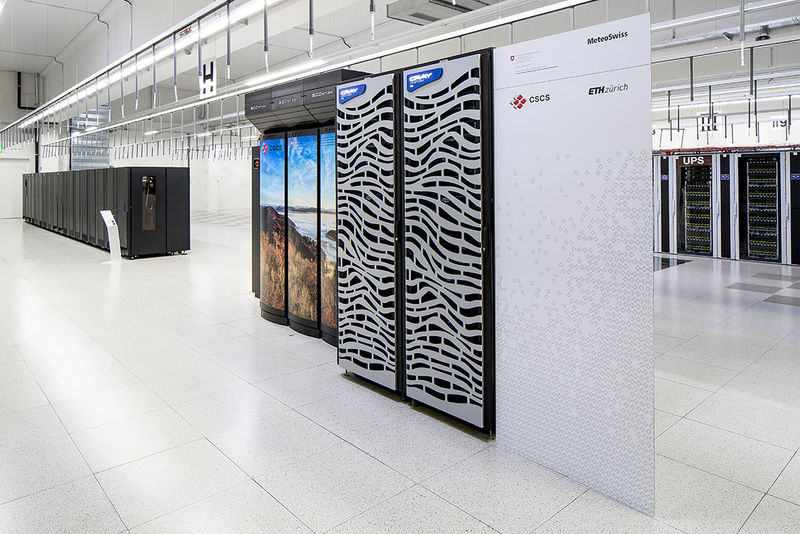
\includegraphics[height=8em]{images/meteoswiss-computer1.jpg}
		\label{fig:meteoswiss-computer1}
	\end{minipage}
	\begin{minipage}{.5\columnwidth}
		\centering
		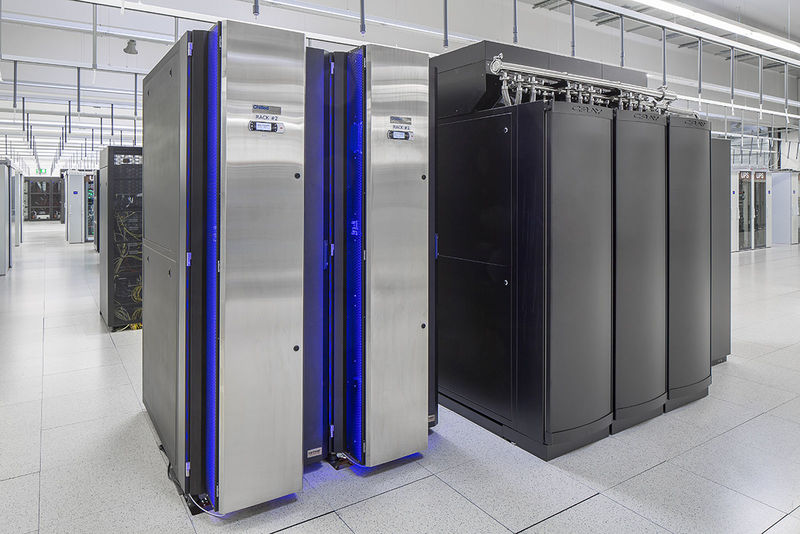
\includegraphics[height=8em]{images/meteoswiss-computer2.jpg}
		\label{fig:meteoswiss-computer2}
	\end{minipage}
	\caption{Kesch and Es-cha, the two compute clusters dedicated for the MeteoSwiss weather prediction. \textit{cscs.ch}}
\end{figure}


\subsection{Current Limitation}
Even thought the transistor density and the number of computations per time unit is still increasing, the memory subsystem can not keep up. Stencil computations on structured grids, which COSMOs dynamical core consists of are heavily memory bound. Figure \ref{fig:dycore-estimate-complexity} illustrates the abstraction levels from the dynamical core as a stencil program down to the actual compute stencils with their corresponding data field accesses. This means that the ratio of compute operations compared to the number of data field accesses is very low. This fact limits the effectiveness of the upgrade of compute resources, since many compute elements are idling and waiting for data to be transfered to them. \\
STELLA \cite{label2} and MODESTO \cite{label3} try to solve or mitigate this problem by optimizing the stencil programs to optimally use the cache hierarchy and therefore reducing the stress on the actual memory bandwidth. 
\begin{figure}[H]
	\centering
	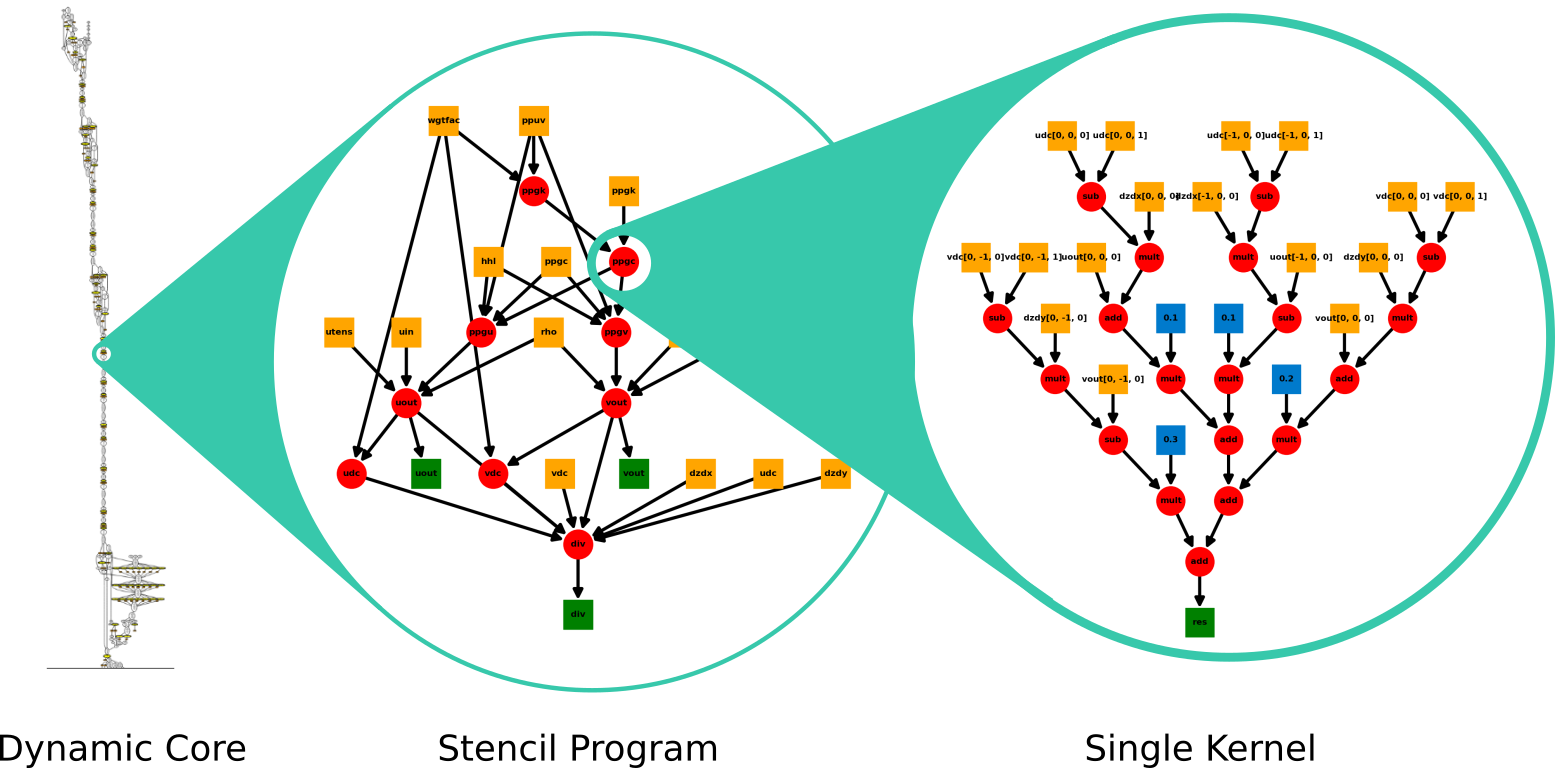
\includegraphics[width=.7\textwidth]{drawings/dycore-estimate-complexity.png}
	\caption{Overview of the total complexity and number of memory accesses given the different hierarchy layers of abstraction.}
	\label{fig:dycore-estimate-complexity}
\end{figure}


\subparagraph{Benefit of FPGA}
This is exactly where the strength of FPGAs lies in. The freedom of not having fixed, hard-wired cache hierarchies, but rather access to spread the fast memory resources in a fine-grained manner such that the overall design profits the most. This increases the actual number of computations per unit time. The next chapter is dedicated to our solution approach and how we intend to implement this in practice.